\documentclass[journal=jprobs,manuscript=article]{achemso}

\usepackage[version=3]{mhchem} % Formula subscripts using \ce{}
\usepackage[T1]{fontenc}       % Use modern font encodings
\usepackage{multirow}
\usepackage{subcaption}
\usepackage{booktabs}
\usepackage{hyperref}

\newcommand*\mycommand[1]{\texttt{\emph{#1}}}

\author{Stefan K. Solntsev}
\email{solntsev@wisc.edu}
\author{Michael R. Shortreed}
\author{Brian L. Frey}
\author{Lloyd M. Smith}
\affiliation[UwMadison]
{University of Wisconsin-Madison}
	
\title[Rapid and Accurate Global PTM Discovery (G-PTM-D) Using Post-Acquisition Spectral Calibration and Multi-Notch Searches]
  {Rapid and Accurate Global PTM Discovery (G-PTM-D) Using Post-Acquisition Spectral Calibration and Multi-Notch Searches}

\begin{document}

\begin{abstract}

Correct identification of protein post-translational modifications (PTMs) is crucial to understanding many aspects of protein function in biological processes.
G-PTM-D\citep{Li_2016} is a recently developed tool for global identification and localization of PTMs.
Spectral file calibration prior to applying G-PTM-D, and algorithmic enhancements in the peptide database search shown here significantly increase the accuracy and speed of PTM identification.
We enhance G-PTM-D by using targeted multi-notch searches, and demonstrate its effectiveness in identification of numerous types of PTMs, including high-mass modifications such as glycosylations.
The changes described in this work lead to a 20\% increase in the number of identified modifications and an order of magnitude decrease in the search time.
Targeted multi-notch searches are also shown to be useful in contexts other than G-PTM-D, producing superior results when used instead of standard narrow-mass and wide-mass searches.
\end{abstract}

\section{Introduction}

Many types of post-translational modifications (PTMs) are known, and databases containing detailed information about such modifications are readily available\citep{Creasy_2004}.
Information about a modification often includes the chemical or isotopic composition, mass, specificity to certain residues, and possible restriction of placement to peptide or protein termini.
Protein databases such as UniProt include information on the localization of specific modifications to specific residues in the protein, but this information is incomplete.
Despite the extensive cataloging of the different possible protein modifications, their comprehensive discovery and identification in complex biological samples has continued to pose a challenge for proteomics\citep{Olsen_2013}.

Numerous procedures for identification and localization of PTMs from "bottom-up" tandem mass spectrometric datasets exist, and those address primarily common modifications (e.g. phosphorylations) in well-studied systems.
Global discovery tools, such as MODa\citep{Na_2011} are also available.
G-PTM-D\citep{Li_2016} is one recently described bioinformatics tool for high confidence identification and localization of a wide variety of different PTMs.
The G-PTM-D workflow consists of three stages: 1) A wide-mass database search\citep{Chick_2015, Na_2011}, that provides mass differences between the identified peptides and the observed precursor peptide masses (hypothesized to differ in mass due to the presence of a PTM);
2) For those peptides for which the mass difference corresponds to the mass of a known PTM, a database augmentation step adds plausible localized PTMs to the corresponding protein entries in the search database;
3) A final standard narrow-mass search of the augmented database to identify both modified and unmodified peptides subject to the standard FDR threshold (e.g. 1\% FDR).

As described above, G-PTM-D has a few significant limitations.
The initial wide-mass search procedure is slow, taking hours for modest size datasets.
Due to this, high mass modifications, such as glycosylations are out of reach, since widening the search window from the suggested $\pm 200$ Da increases the search time even more.
The final narrow-mass search is also problematic, since it does not account for peptide-spectral matches(PSMs) with mass differences arising due to misidentifying the monoisotopic peak.
In G-PTM-D, modification discovery is limited to PTMs in the Uniprot database: this is a significant limitation since that database does not include modifications arising from sample handling, and ignoring those modifications significantly degrades the final PTM identification rates.
Finally, PTMs that are similar in mass, such as phosphorylation (79.966331 Da) and sulfonation (79.956815 Da), are problematic since they are virtually indistinguishable in unprocessed spectral files.
These limitations motivated the work described here.

Spectral calibration is essential for distinguishing modifications with similar mass, so we recommend running the G-PTM-D procedure only on calibrated spectra files.
To address the long search times of the wide-mass search, we replace the wide-mass search in the first stage by a specialized search called a multi-notch search that only allows specific mass differences which correspond to pre-selected modification masses (e.g. PTMs and amino acids).
This change improves the specificity of the search and significantly decreases search time.
The final narrow-mass search is also replaced by a limited multi-notch search that accommodates errors in precursor mass deconvolution (+1.0029, + 2.0052 and + 3.0077 Da), further increasing the number of confidently identified peptides and PTMs.
Finally, we replace the limited Uniprot PTM list with a customizeable expanded list of modifications that includes chemical adducts, glycosylations, lipids, and other important modifications.
This change not only expands the list of identified and localized modifications, but also indirectly improves the confident PSM count.
The enhanced G-PTM-D workflow is presented in Figure~\ref{fgr:diagram}.

\begin{figure}[H]
  \includegraphics{paperDiagram.png}
  \caption{The three steps of the G-PTM-D workflow are indicated in the light beige color.}
  \label{fgr:diagram}
\end{figure}


\section{Experimental Procedures}

We developed a modified version of the Morpheus software for bottom-up spectral database searching\citep{Wenger_2013} that we call MetaMorpheus\footnote{Free and Open Source software available at \url{https://github.com/smith-chem-wisc/MetaMorpheus}}, which integrates the database search procedure with spectral calibration and the enhanced G-PTM-D workflow.
Three multi-fraction mammalian datasets (Jurkat cell, C57BL/6J (B6) and CAST/EiJ (CAST) mouse islet lysates) with deep proteome coverage were used to evaluate performance.
These tryptically digested cell lysates correspond to 28 fractions from human Jurkat cells, and 18 fractions from Mouse islets, and are described in detail in~\citep{Shortreed_2015, Cesnik_2016}.

Uniprot XML protein databases acquired on Feb 27, 2017 containing only reviewed human/mouse proteins were employed.

A 10ppm precursor mass tolerance is used for the initial calibration step, and then reduced to 5ppm for subsequent searches.
We allowed 120 modifications including PTMs, adducts, and chemical modifications in the database augmentation step.

\section{Results and Discussion}

This work presents four major changes to the previously published G-PTM-D workflow:
a spectral calibration;
a replacement of the wide parent mass tolerance search with a custom multi-notch search for PTM discovery;
replacement of the final traditional narrow mass search with a limited multi-notch search that permits identification of incorrectly deconvoluted precursor masses;
and lastly, addition of capacity for identification of multiple cofragmented peptides from a single MS/MS scan.
To clarify the advantage of each change, they are first discussed separately, followed by an analysis of their combined effect upon overall G-PTM-D performance.

\subsection{Calibration}

A critical parameter for peptide identification is mass accuracy\citep{Scherl_2008}.
Higher mass accuracy provides increased specificity and thus confidence in peptide identifications, decreasing the false discovery rate.
Instrument noise, systemic drift and miscalibration limit the mass accuracy in acquired spectra.
Multiple calibration strategies to improve mass accuracy have been devised, and fall into three general categories: External calibration prior to the MS experiment (e.g. standard instrument calibration protocols); internal calibration during the MS experiment (e.g. real-time calibration using a lock mass standard\citep{Olsen_2005}); and spectral calibration subsequent to the MS experiment (post-acquisition spectral calibration).
We developed a post-acquisition calibration procedure that builds upon the software lock mass concept\citep{Cox_2011} recently reported by the Mann group.
In our strategy, the m/z differences between expected and observed peaks in the peptide tandem ms spectra are compiled, and then used to recalibrate the spectra.
The spectral calibration procedure consists of two steps: Step 1: A narrow tolerance (e.g. 10 ppm precursor, 0.01 Dalton fragment) database search is performed on the dataset.
This yields a set of peptide identifications subject to a desired false discovery rate (e.g 1\%; based upon the target:decoy strategy\citep{Elias_2007}).
Step 2: The identifications from Step 1 are used to extract peak matches from the spectra, and a peak shifting procedure is performed.
The calibration algorithm is described in detail in Supplementary Material 1.

Calibration quality is evaluated through the results of a standard 10ppm precursor tolerance database search.
PSMs within 1\% FDR prior to calibration are compared with PSMs after the calibration procedure (Table~\ref{tbl:calib}).
The calibration procedure successfully addresses instrument miscalibration by centering the average error around zero.
The systemic noise introduced by various other factors is also addressed: this is evident in the decrease in the standard deviation of the errors in the precursor mass estimates, which show that the calibrated mass spectra have sub-ppm mass errors.
Histograms of the mass errors before and after calibration are plotted in Figure~\ref{fgr:figure1}.

\begin{table}[]
\centering
\caption{PSMs Within 1\% FDR Before and After Calibration}
\label{tbl:calib}
\begin{tabular}{@{}llllll@{}}
                                                                                &        & \multicolumn{2}{l}{Mouse} & \multicolumn{2}{l}{Jurkat} \\ \cmidrule(l){3-6} 
                                                                                &        & Orig        & Calib       & Orig        & Calib        \\ \cmidrule(l){3-6} 
\multicolumn{2}{l}{PSM Count}                                                            &    152208       &        155617 &         217612   &   219172        \\
\multicolumn{2}{l}{Average Error (ppm)}                                                           &    -1.09         &       -0.16      &      -2.10      &        -0.16      \\
\multicolumn{2}{l}{St. Dev of Error}                                                     &     3.35        &      0.90       &       2.15      &        0.91      \\
\multirow{3}{*}{\begin{tabular}[c]{@{}l@{}}Confidence\\ Intervals\end{tabular}} & 68.3\% &   [-4.44,2.27]          &    [-1.06,0.74]          &    [-4.26,0.05]          &  [-1.08,0.75]            \\
                                                                                & 95.4\% &   [-7.80,5.62]          &    [-1.97,1.64]         &   [-6.41,2.20]          &      [-1.99,1.61]         \\
                                                                                & 99.7\% &   [-11.15,8.98]          &      [-2.87,2.54]        &    [-8.56,4.36]          &      [-2.90,2.58]         \\ \cmidrule(l){3-6} 
\end{tabular}
\end{table}

%\begin{figure}
%  \includegraphics{calib1.png}
 % \caption{Histograms demonstrating the effect of calibration on PSM mass errors}
 % \label{fgr:figure1}
%\end{figure}

\newpage

\subsection{Multi-Notch Searches}

Prior to discussing the impact that multi-notch searches have on the G-PTM-D performance, it is useful to describe the variety of search tolerances used.
Traditional searches in bottom-up proteomics score potential matches between theoretical peptides and experimental spectra if the candidate peptide mass and the observed precursor mass are equal, within some defined tolerance (e.g. 5ppm, or 2.1 Da).
We'll refer to this type of search here as a \textit{single-notch} search.
The other common search mode, used in the original G-PTM-D publication, is a \textit{wide-parent tolerance search} ($\pm 500$ Da).
In that search, the precursor mass and the mass of the best matching theoretical peptide could be many Da apart.
An even less restrictive \textit{open-mass} search, matches peptides from a database to fragmentation spectra without taking the precursor mass into account at all.
We describe an alternative to these search modes: the multi-notch search.
The \textit{multi-notch} search is an extension of the single-notch search to multiple specific mass differences between precursor mass and theoretical mass~\ref{fig:fig1-searchtypes} where the mass difference is easily interpretable.
It can also be seen as a narrowing of the wide-parent tolerance search to only include pre-specified mass differences.
The advantages and disadvantages of this alternative strategy are described below.

%\begin{figure}
%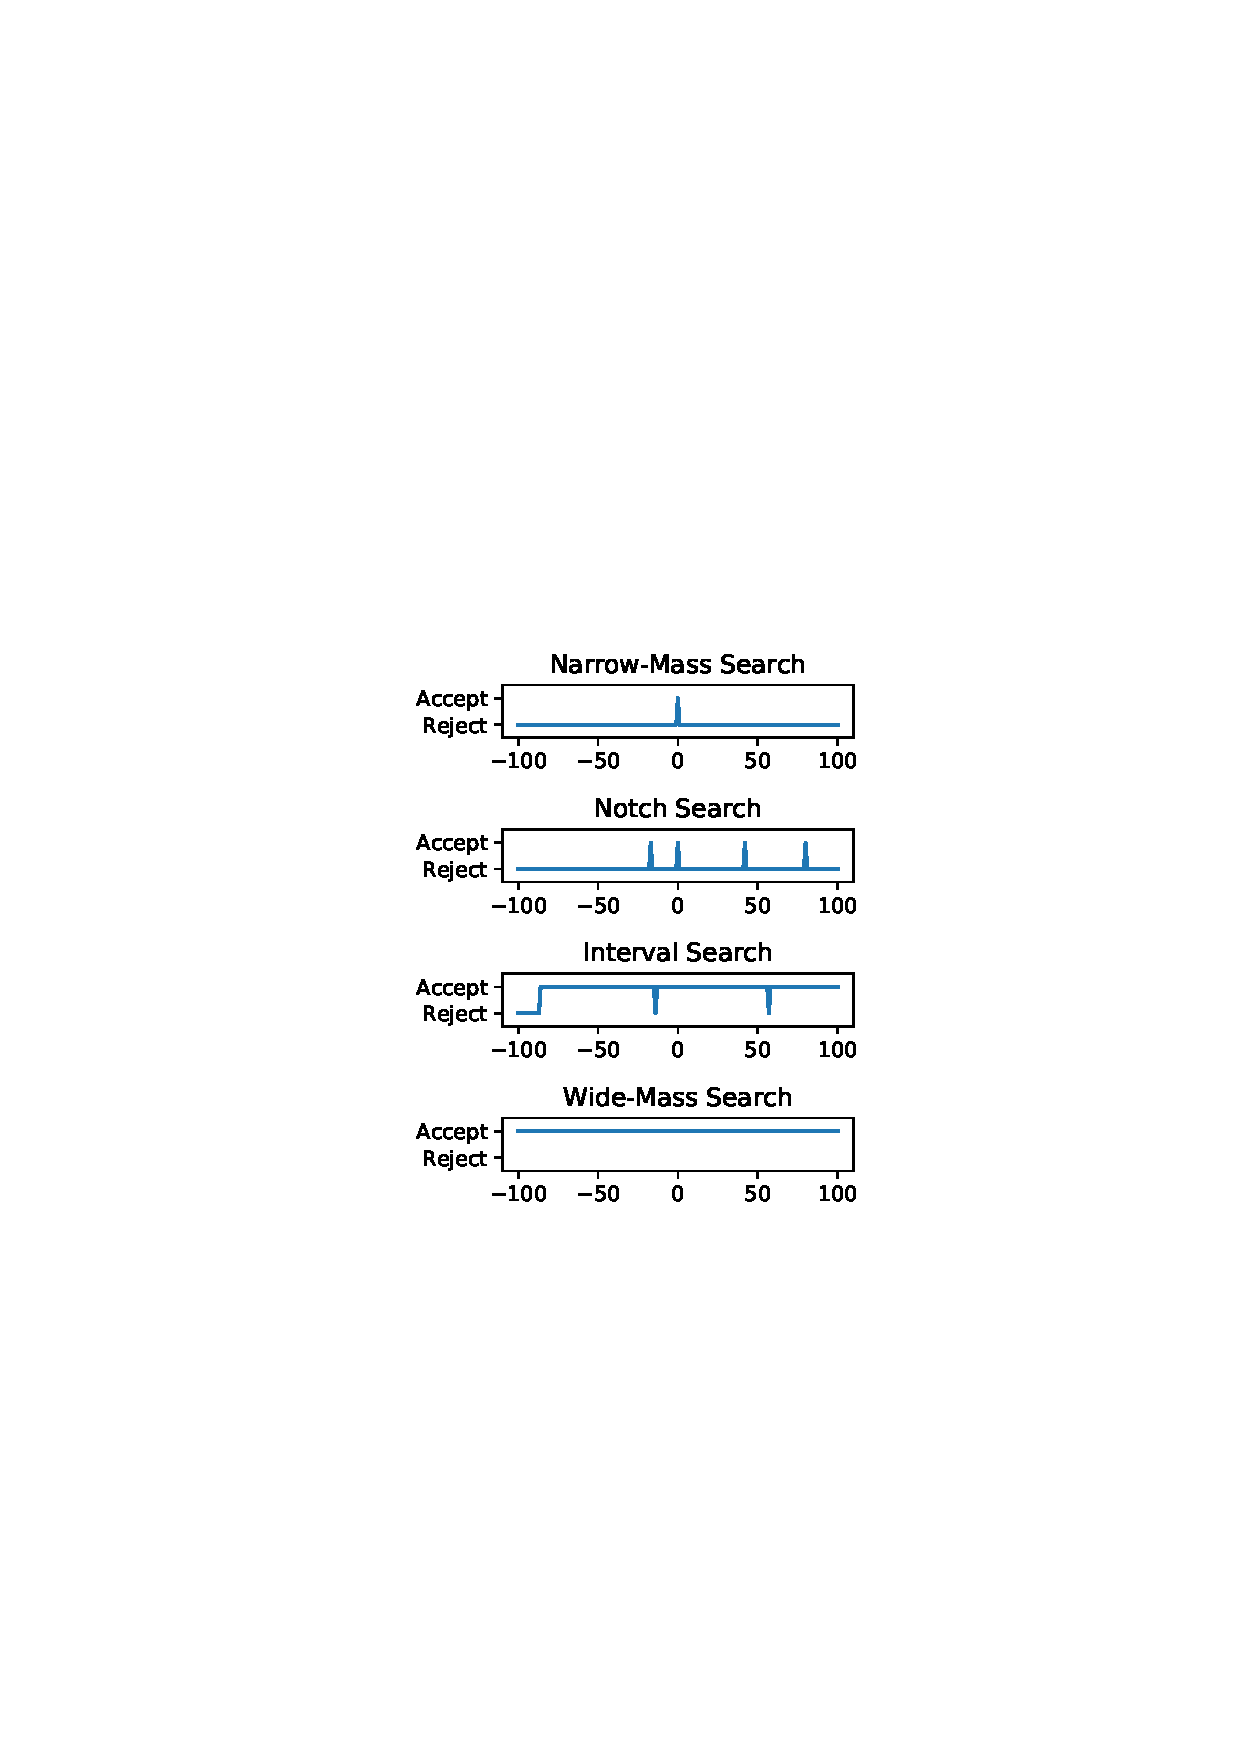
\includegraphics{fig1-searchTypes.png}
%\caption{Search Modes}
%\label{fig:fig1-searchtypes}
%\end{figure}

\subsubsection{Traditional Single-Notch Search vs. Limited Multi-Notch Search}

The traditional single-notch search limits the range of acceptable mass differences between a candidate peptide and the observed experimental precursor in order to find an exact match to the observed peptide in a protein database.
A mass tolerance of 5-20ppm is a common precursor mass tolerance that allows only mass differences between theoretical and experimental of 5-20 ppm.
This is a highly restrictive search.
It is not uncommon for the precursor mass tolerance of single-notch searches to be reduced to as much as 2 or 3 Da.
One rationale for this is that errors in the deconvolution of MS1 spectra frequently result in an experimental precursor mass that is in error by 1-3 Da, corresponding to missed monoisotopic errors.
This relaxed tolerance increases the number of correctly identified peptides.
A second rationale for this approach is that multiple peptides are frequently co-isolated and co-fragmented with all peptide fragments being reported in the same tandem mass spectrum.
Frequently a peptide with a mass differing from the precursor mass reported by the instrument is the identified peptide.
In case the co-fragmented peptides have the same charge, the mass difference between the identified peptide and the isolated precursor can be as much as 2 or 3 Da, so a lose 2 or 3 Da tolerance is able to identify those.
The major limitation to this relaxed parent mass tolerance is a significant increase in the number of false positive identifications (due to a vast expansion in the number of acceptable theoretical peptides and simultaneous failure to accommodate low mass modifications such as amidation and deamidation), arguably defeating the purpose of a narrow-mass search.
 
An alternative to these two traditional single-notch searches is a limited multi-notch search that allows mass differences between precursor and theoretical peptide of 0, 1.0029, 2.0051 or 3.0077 Da but limits the width about any one of those three tolerances to a few ppm (0-20 ppm).
This approach provides a means of getting an increased number of correct identifications but mitigates problems with false positive identifications.
This alternative would appear to result in loss of identification of co-isolated peptides.
However, MetaMorpheus was programmed to ignore the precursor mass reported by the mass spectrometer in the mass spectrum and instead, deconvolute all peaks in the MS1 spectrum associated with the tandem mass spectrum to recover all possible precursor masses.
This expanded list of precursors is used in every spectrum match frequently resulting in multiple peptide identifications from single tandem mass spectrum.  


INSERT PARAGRAPH DESCRIBING RESULTS OF SINGLE NOTCH VERSUS LIMITED MULTI NOTCH \& COISOLATION


We observe that when using an incomplete database that does not include comprehensive modification and sequence variation information, a notch search with notches at monoisotopic peaks is superior to either of the single-notch searches.


\begin{table}[]
\centering
\caption{Notch Search vs Narrow-Mass Search comparison of PSMs for Mouse}
\label{my-label}
\begin{tabular}{@{}llll@{}}
                    & 5ppm Search & 3.5 Da Search & Notch Search \\ \cmidrule(l){2-4}
PSMs Within 1\% FDR & 157188      & 178003        &        \\
MisAssigned PSMs    & 0           &               & 0            \\
Good PSMs           & 157188      &         &        \\ 
\end{tabular}
\end{table}

%\begin{figure}
%\caption{Mouse histograms around 0}
%\label{fig:fig3mouse-1012}
%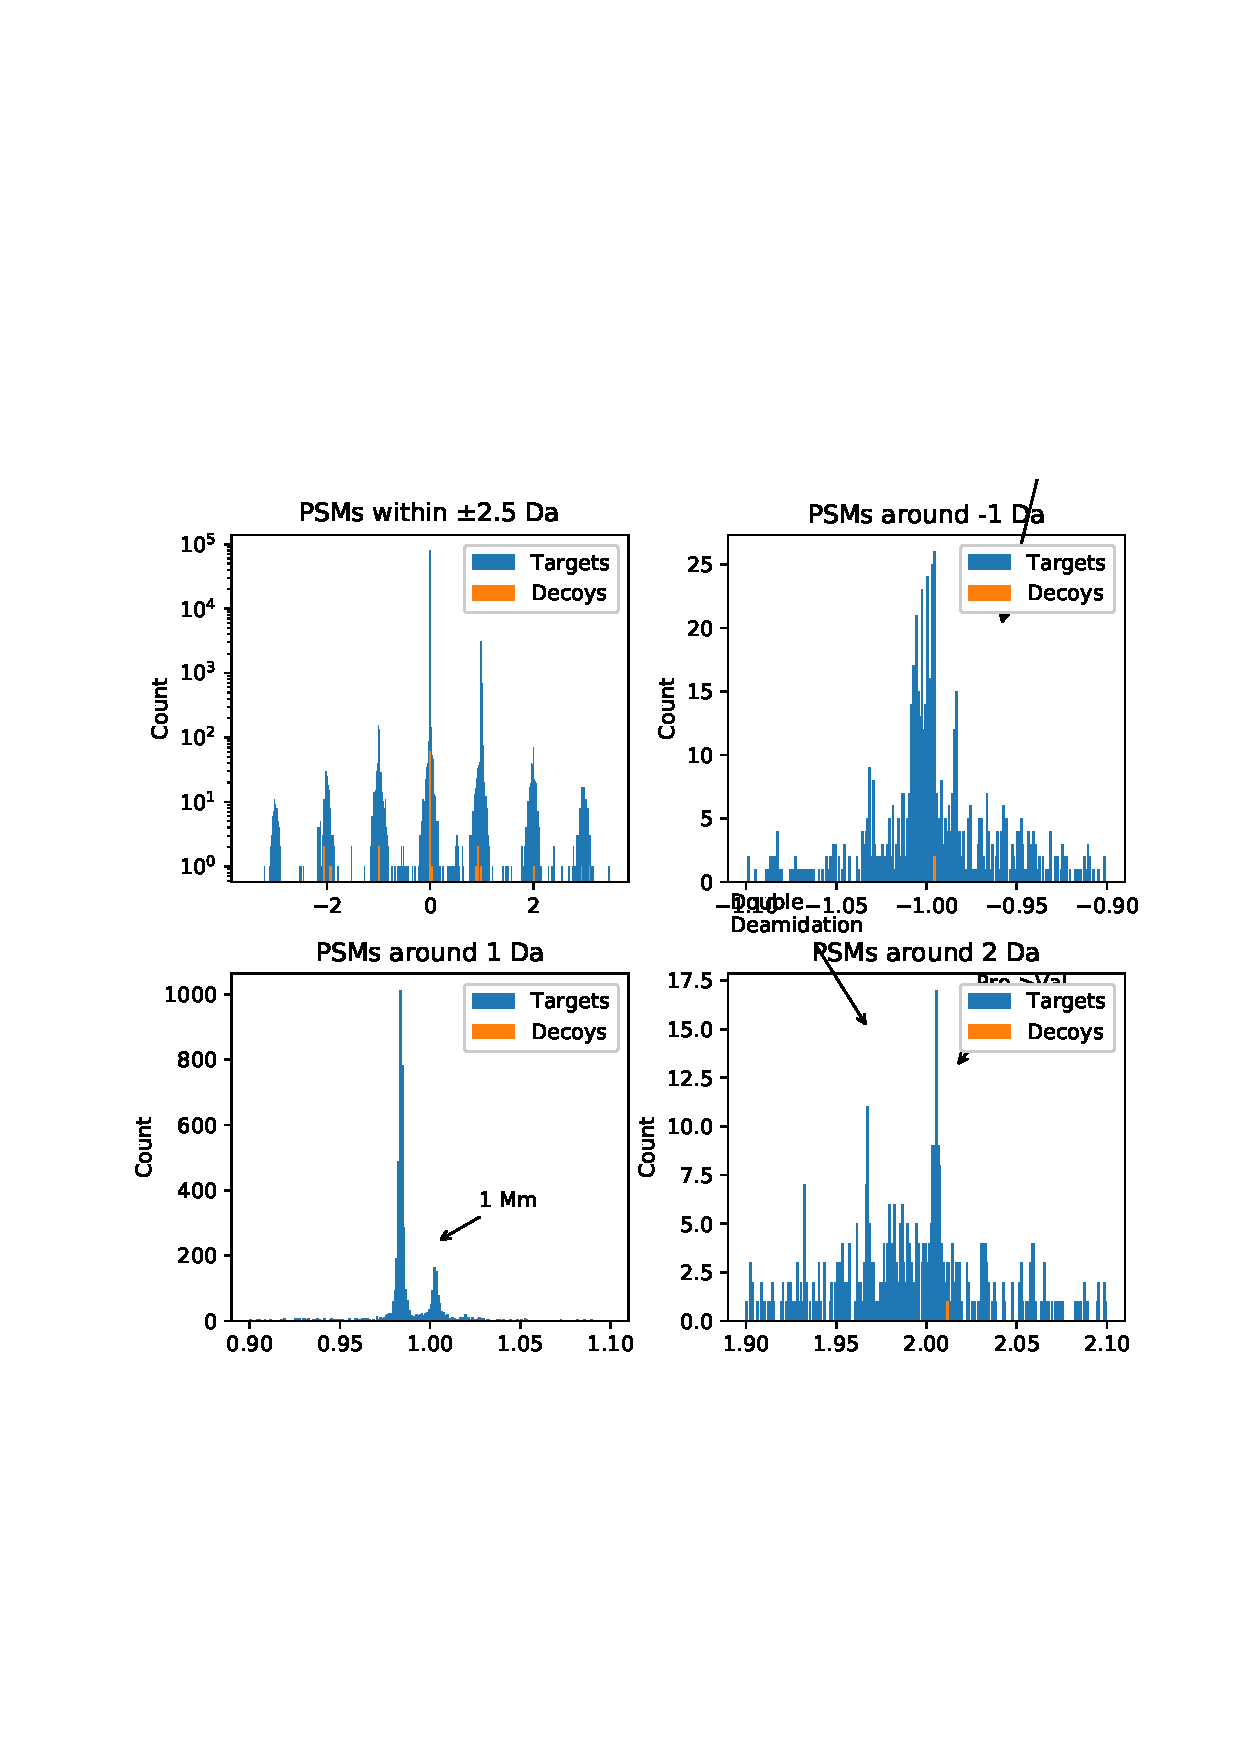
\includegraphics{fig3mouse-1012.png}
%\end{figure}

%\begin{figure}
%\caption{Jurkat histograms around 0}
%\label{fig:fig3jurkat-1012}
%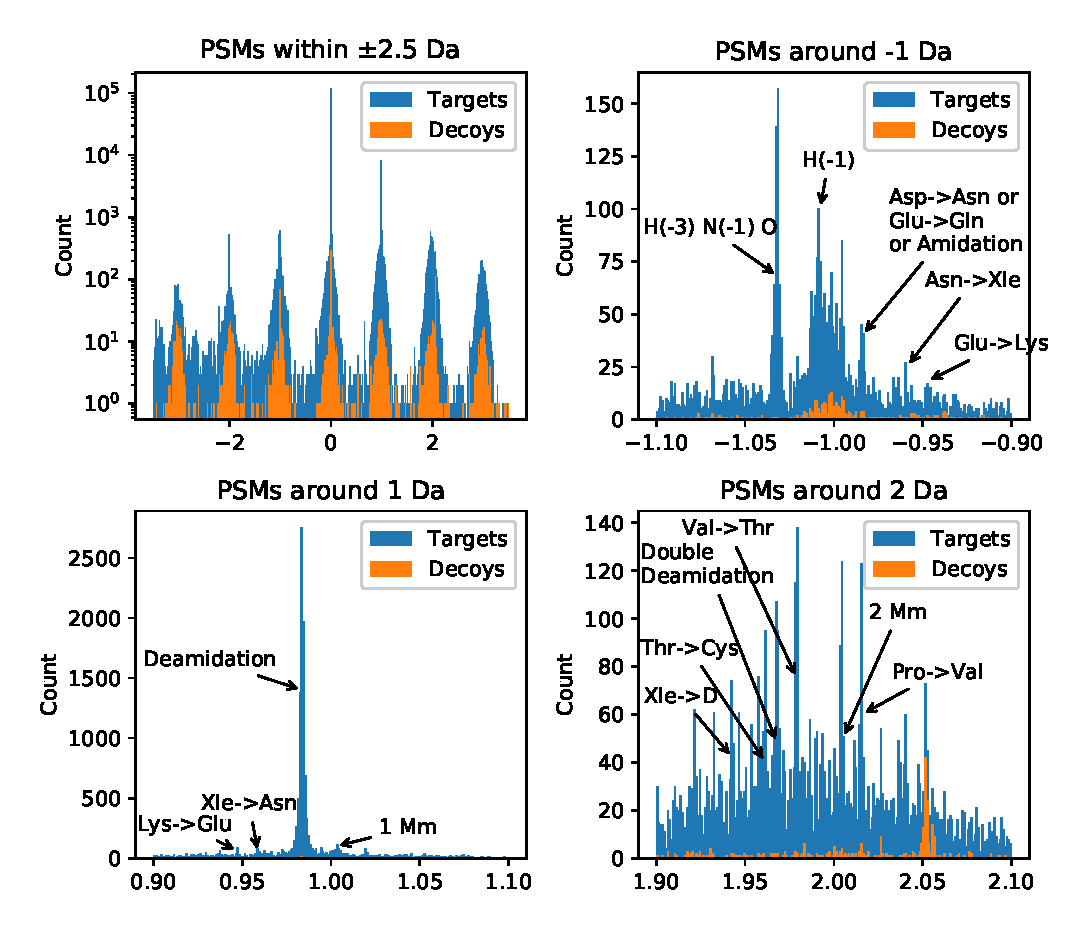
\includegraphics{fig3jurkat-1012.eps}
%\end{figure}

\subsubsection{Multi-Notch Search vs. Wide-Mass Search}

Chick~\citep{Chick_2015} showed that by significantly relaxing the parent mass tolerance in bottom-up searches, an incredible variety of unforeseen peptides were being fragmented and could be identified.
In particular, PTM-containing peptides could be identified from those MS2 fragments that did not possess the modification and the type of PTM could be inferred from differences in precursor and parent mass.
A major limitation of the Chick work was the extremely long search times because of the vast number of theoretical candidate peptides that were evaluated for each and every MS2 spectrum.
Recently, Kong\citep{Kong_2017} reported a new index-based search strategy (MSFragger) that radically improved search speeds for wide parent mass tolerance searches.
Search times for +/- 500 Da parent tolerances went from six years to six seconds.
The output of both search strategies is a list of PSMs, where the best matching unmodified theoretical peptide was found for each MS2 fragmentation spectrum and the mass difference between the theoretical and experimental precursor masses was determined.
The mass differences can be clustered into histogram peaks\citep{Rodriguez_2014}, but interpretation of the mass difference was left to the user.
PTMs corresponding to the reported mass difference can frequently be inferred; such as when the mass difference reported matches a known PTM mass (e.g. 79.966331 Da for phosphorylation).
However, mass differences can arise from not only one modification, but frequently from two or more modifications, some of which increase the mass and the peptide and some of which decrease it. In addition, small missed cleavages are sometimes reported mistakenly as mass differences. Also, some mass differences, such as those matching to amino acid masses, are easily interpreted but suffer from high local FDR and should only be used with caution. Finally, seemingly uninterpretable mass differences can be reported when the best matching peptide has an actual precursor mass different from the precursor mass selected by the mass spectrometer. The range of masses selected for fragmentation in a tandem mass spectrometer is commonly +/- 2 Da. Therefore, multiple peptides can be introduced to the cell and co-fragmented. This often results in peptide identification of a less abundant peptide with mass slightly larger or smaller than the selected precursor.
The unconstrained utilization of mass difference and acceptance of the theoretical best matching sequence as true can result in a high number of false positive assignments. 

A third alternative, reported here, is the use of a multi-notch search (>100 discrete notches) offers a means of reducing the search space and limiting the number of theoretical candidates to those plausible for the scan, increasing the search speed and most importantly, producing the most correct PSMs and the least false positive PSMs (see the TABLE i and TABLE j).
	Table I (Count of theoretical peptide candidates for each search mode (single notch 5ppm, single notch 3.5, limited multi notch, 500 Da, and full multi-notch).
	Table J (Total PSMs for each search type – 500 or full multi-notch). 
One output of an MSFragger search is a list of PSMs with each entry containing the mass difference between the isolated precursor and the mass of the best matching theoretical peptide. MSFragger also doesn’t automatically calibrate spectra prior to searching. Therefore, mass differences from closely spaced PTMs (e.g. phosphorylation and sulfonation) can easily be misinterpreted. MetaMorpheus has built in functionality to identify multiple peptides from each tandem mass spectrum resulting in improved identification of peptides and peptide modifications.


G-PTM-D originally added PTMs with masses that were included in the UniProt ptmlist… We have since increased the variety of PTMs added but including a number of new notches in the G-PTM-D first pass search. The new notches correspond to metal adducts (e.g. Na and K), glycoslyations, sample handling and processing artifacts (e.g. carbamylation, ammonia loss), lipidation, and etc. 
Msfragger has limited mass range as reported.
We identified peaks with anomalously high false discovery rates, which could be excluded from wide mass searches in order to improve the overall identification quality. Some of these problematic histogram peaks are illustrated in Figure [fig:figure3], including peaks corresponding to masses of Sulfo and Phospho, and a problematic peak at mass of Leucine, with a high FDR .
Some Histogram Peaks For Mouse Data
Some Histogram Peaks For Mouse Data
We identified some specific mass shifts that are characterized by anomalously high false discovery rates: these mass shifts correspond precisely to various combinations of residue mass additions and removals .

\subsection{Enhanced G-PTM-D Results}

A major improvement in G-PTM-D performance arises from using calibrated spectra as inputs to the procedure. 
Calibration and the associated increase in mass accuracy is essential for discrimination of small differences between mass shifts due to different modifications.
To illustrate this, mass shifts around 80 Daltons from the initial notch search are aggregated in the histograms in Figure~\ref{fig:phosphoHistograms}.
It is evident from these histograms that the phosphorylation and sulfonation peaks are clearly separated and identifiable when the search is conducted on well-calibrated spectra.

%\begin{figure}	
%	\centering
%	\begin{subfigure}[t]{3.1in}
%		\centering
%		\includegraphics[scale=0.5]{figPhosphorylationPre.png}
	%	\label{fig:1a}		
%	\end{subfigure}
%	\quad
%	\begin{subfigure}[t]{3.1in}
%		\centering
%		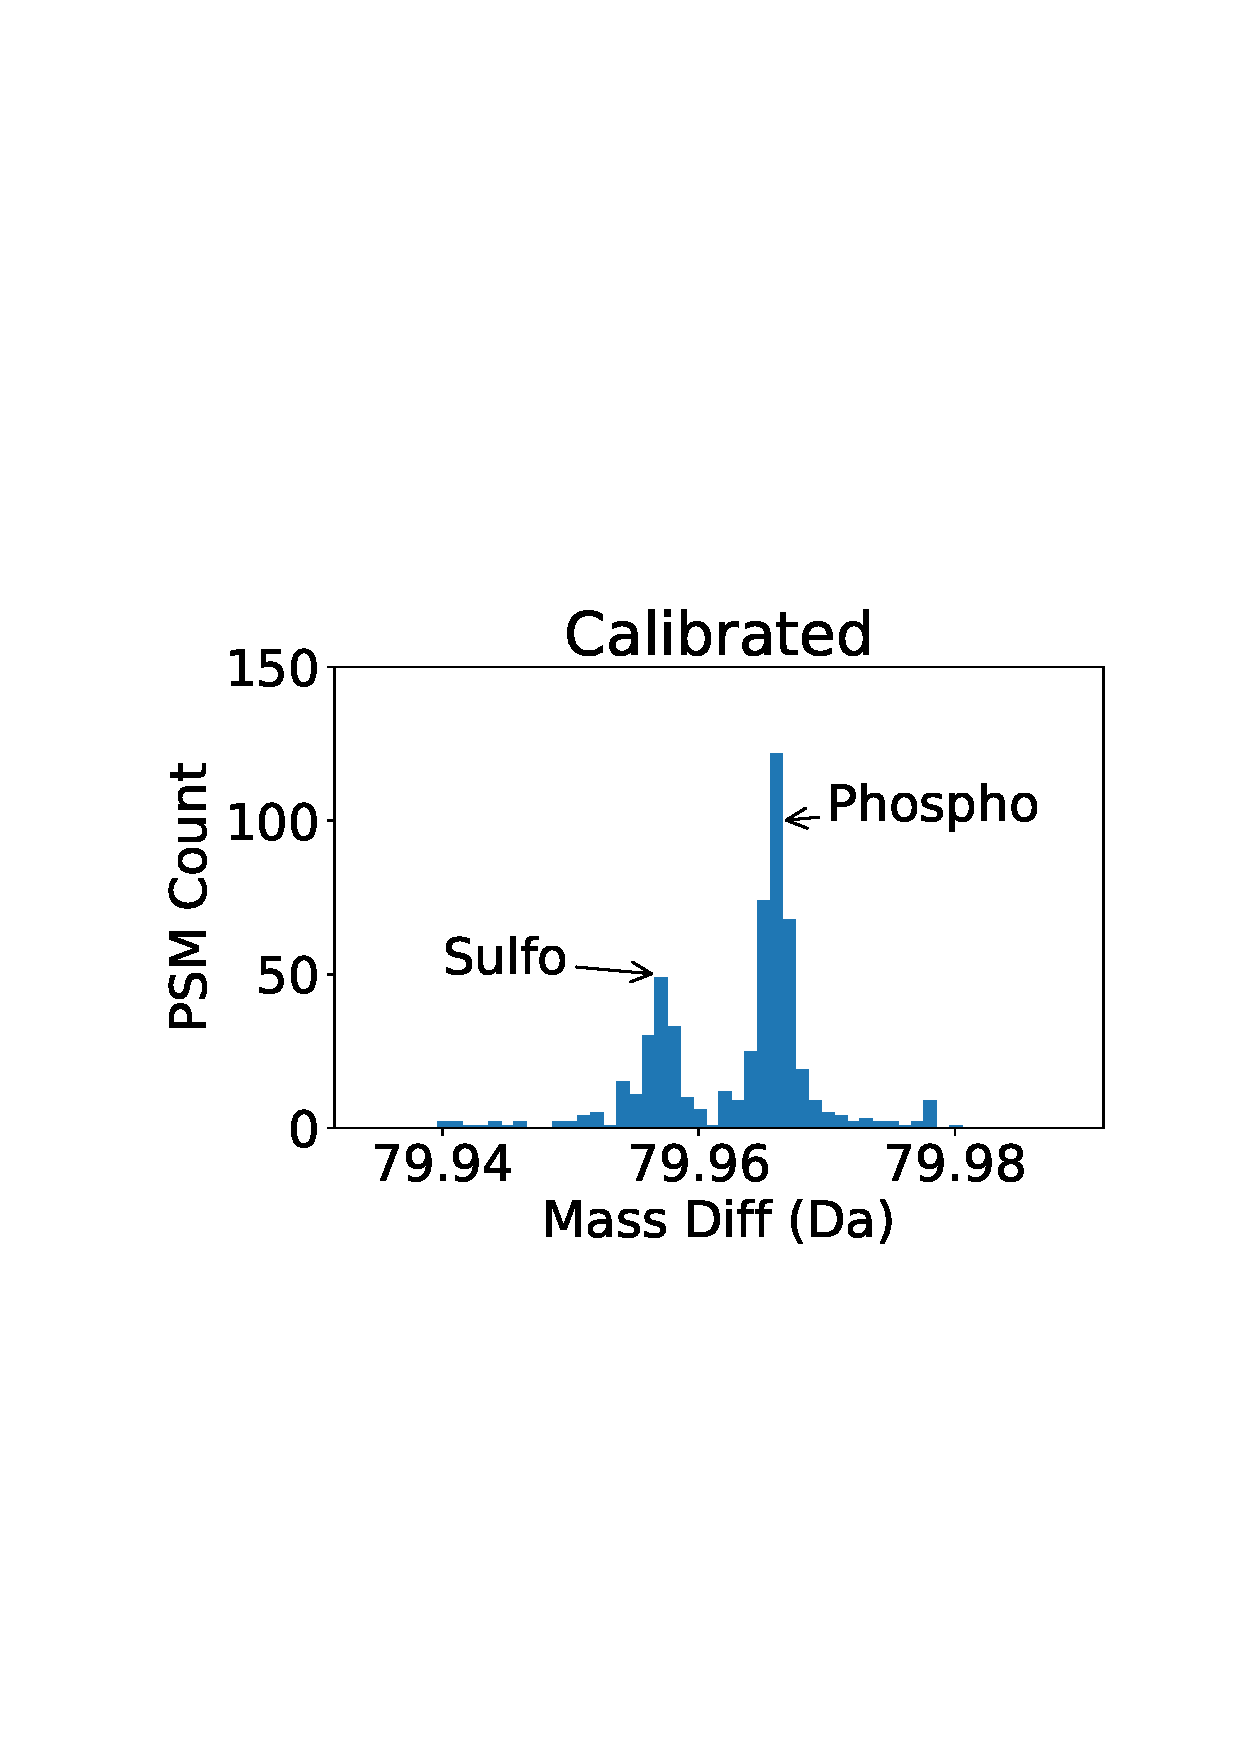
\includegraphics[scale=0.5]{figPhosphorylationCalib.png}
%		\label{fig:1b}
%	\end{subfigure}
%	\caption{Histograms of mass differences observed around 80 Daltons when using calibrated and uncalibrated %spectra}\label{fig:phosphoHistograms}
%\end{figure}

By employing the novel notch search strategy instead of the wide-mass search in the G-PTM-D process, using only the modifications listed in Uniprot, the number of confidently identified PSMs increased by 6\%.
The overall search time dropped significantly, from 35 hours to 4 hours for all datasets, see Table~\ref{my-labelff}.

\begin{table}[]
\centering
\caption{Effects of Replacing Initial Wide-Mass Search by a Multi-Notch Search}
\label{my-labelff}
\begin{tabular}{ll|l|l}
                      &        & Wide-Mass Search & Notch Search\\
\hline
\multirow{2}{*}{Time} & Jurkat & 22.1 hrs         & 2.9 hrs    \\
                      & Mouse  & 13.5 hrs         & 1.2 hrs   \\
\hline
\multirow{2}{*}{PSMs} & Jurkat & 203237           & 210566    \\
                      & Mouse  & 153674           & 162473   
\end{tabular}
\end{table}


The final notch search uses notches centered at \{0, 1.0029, 2.0052, 3.0077\}, in order to capture missed identifications due to missed monoisotopic peaks.
The results are contrasted with the standard narrow-mass final search.
The effect of using these notches is shown in Table~\ref{tab:table2}.

\begin{table}[]
\centering
\caption{Effects of Replacing Final Narrow-Mass Search by a Notch Search}
\label{tab:table2}
\begin{tabular}{ll|l|l}
                      &        & Narrow-Mass Search & Notch Search\\
\hline
\multirow{2}{*}{PSMs} & Jurkat  & 210566   &  220574  \\
                      & Mouse    & 162473   &   170743
\end{tabular}
\end{table}

Since the protein database is annotated with PTMs from the UniProt PTM list, it is natural to use it in the augmentation step as well.
It has a few significant drawbacks: Some mass values do not correspond to actual mass shifts, lability of modifications is not taken into account, and many PTMs are missing, including adducts and glycosylations.
Notch searches allow using expanded modification lists that include chemical modifications such as adducts and large mass PTMs such as glycosylations.
Even though adducts arising from experimental artifacts are not ultimately interesting to biologists, not including them as an option decreases the total number of identified proteins and PTMs.
A curated set of notches and the corresponding modifications is given in Appendix A.
The overall identification rate increased from 164,697 to 179,345 peptide-spectral matches (PSMs), which in turn increased the number of modified peptides by an additional 20\%.
We identified hundreds of glycosylated peptides in these unenriched samples, with many of these modifications exceeding 1000 Da.

\begin{table}[]
\centering
\caption{Effects of Using Different Modification Lists}
\label{tab:table3}
\begin{tabular}{ll|l|l|l}
                      &        & Only Uniprot & Uniprot+Glyco & Uniprot+Glyco+Adducts\\
\hline
\multirow{2}{*}{PSMs} & Jurkat  & 220574   &  222985 & 223578\\
                      & Mouse    & 170743   &   171432& 174783 
\end{tabular}
\end{table}


%
\begin{acknowledgement}

The authors thank \ldots
\end{acknowledgement}

\begin{suppinfo}

The following files are available free of charge.
\begin{itemize}
  \item Filename: brief description
  \item Filename: brief description
\end{itemize}

\end{suppinfo}

\newpage

\bibliography{citations}

\end{document}
